% TikZ Free Body Diagram: Skydiver with parachute
% Latexdraw.com
% 15:11, 01:05:2020 

\documentclass[border=0.5cm]{standalone}
\usepackage{tikz}
\usepackage{tikzlings-penguins}

\begin{document}

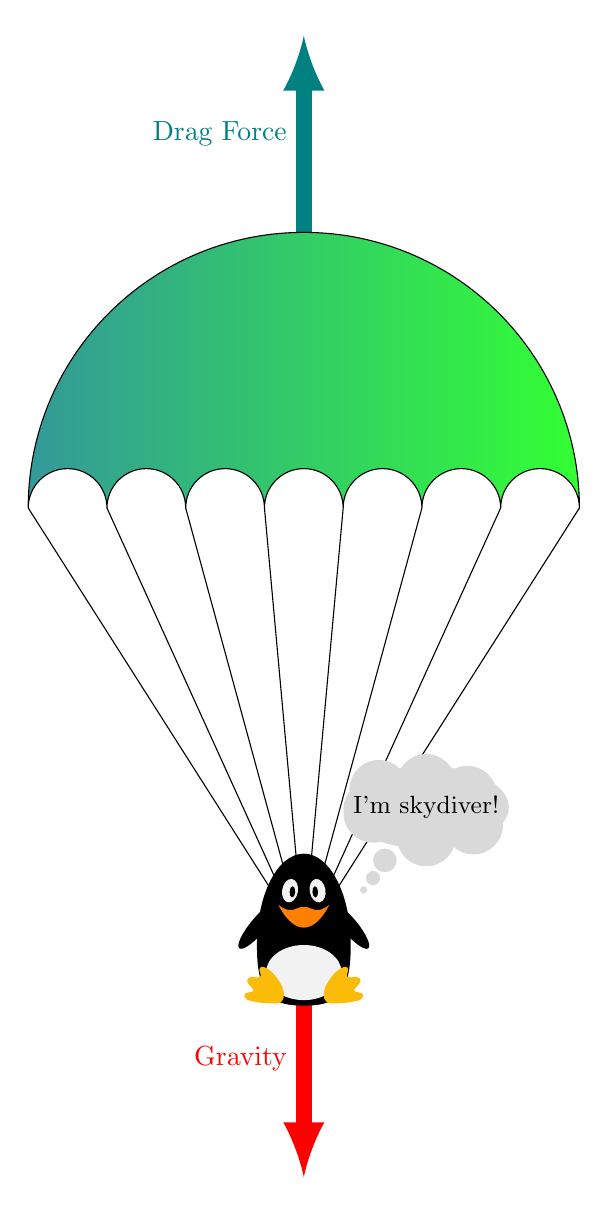
\begin{tikzpicture}

% Free body diagram
% Gravity
\draw[-latex, line width=0.2cm,red] (0,-5.5) -- ++(0,-3cm)
node[midway,left]{Gravity};
% Air resistance force
\draw[-latex, line width=0.2cm,teal] (0,3.5) -- ++(0,2.5cm)
node[midway,left]{Drag Force};

% Canopy
\draw[left color=teal!80,right color=green!80](0:3.5) arc(0:180:3.5)  
\foreach \i in {1,...,7}{arc (180:0:0.5) }-- cycle;

% Suspension lines
\foreach \i in {-3.5,...,3.5} 
{
\draw (\i,0) -- (0,-5.5);
}

% Skydiver (Penguin)
\begin{scope}[yshift=-6.5cm]
\penguin
\thing[
    think={\small I'm skydiver!},
    scale=1.5,
    yshift =-0.6cm,
    xshift=-0.05cm]
\end{scope}

\end{tikzpicture}

\end{document}
